%
% Whitepaper for BlackHat EU 2007 and iSEC website
%
% NOTES:
% listings package reference: http://en.wikibooks.org/wiki/LaTeX/Packages/Listings
%   or ftp://tug.ctan.org/pub/tex-archive/macros/latex/contrib/listings/listings.pdf
% 
% /usr/share/texmf/tex/latex/base/article.cls

\documentclass{article}

% iSEC formatting
%\usepackage{isec_whitepaper}
% epydoc stuff
\usepackage{alltt, parskip, fancyhdr, boxedminipage}
\usepackage{makeidx, multirow, longtable, tocbibind, amssymb}
\usepackage[usenames]{color}
%\setlength{\headheight}{16pt}
%\setlength{\headsep}{24pt}
%\setlength{\topmargin}{-\headsep}
%\setlength{\parindent}{0ex}
%\setlength{\fboxrule}{2\fboxrule}
\newlength{\BCL} % base class length, for base trees.
%\pagestyle{fancy}
%\renewcommand{\sectionmark}[1]{\markboth{#1}{}}
%\renewcommand{\subsectionmark}[1]{\markright{#1}}
\definecolor{py@keywordcolour}{rgb}{1,0.45882,0}
\definecolor{py@stringcolour}{rgb}{0,0.666666,0}
\definecolor{py@commentcolour}{rgb}{1,0,0}
\definecolor{py@ps1colour}{rgb}{0.60784,0,0}
\definecolor{py@ps2colour}{rgb}{0.60784,0,1}
\definecolor{py@inputcolour}{rgb}{0,0,0}
\definecolor{py@outputcolour}{rgb}{0,0,1}
\definecolor{py@exceptcolour}{rgb}{1,0,0}
\definecolor{py@defnamecolour}{rgb}{1,0.5,0.5}
\definecolor{py@builtincolour}{rgb}{0.58039,0,0.58039}
\definecolor{py@identifiercolour}{rgb}{0,0,0}
\definecolor{py@linenumcolour}{rgb}{0.4,0.4,0.4}
\definecolor{py@inputcolour}{rgb}{0,0,0}
% Prompt
\newcommand{\pysrcprompt}[1]{\textcolor{py@ps1colour}{\small\textbf{#1}}}
\newcommand{\pysrcmore}[1]{\textcolor{py@ps2colour}{\small\textbf{#1}}}
% Source code
\newcommand{\pysrckeyword}[1]{\textcolor{py@keywordcolour}{\small\textbf{#1}}}
\newcommand{\pysrcbuiltin}[1]{\textcolor{py@builtincolour}{\small\textbf{#1}}}
\newcommand{\pysrcstring}[1]{\textcolor{py@stringcolour}{\small\textbf{#1}}}
\newcommand{\pysrcdefname}[1]{\textcolor{py@defnamecolour}{\small\textbf{#1}}}
\newcommand{\pysrcother}[1]{\small\textbf{#1}}
% Comments
\newcommand{\pysrccomment}[1]{\textcolor{py@commentcolour}{\small\textbf{#1}}}
% Output
\newcommand{\pysrcoutput}[1]{\textcolor{py@outputcolour}{\small\textbf{#1}}}
% Exceptions
\newcommand{\pysrcexcept}[1]{\textcolor{py@exceptcolour}{\small\textbf{#1}}}
\newenvironment{Ventry}[1]%
 {\begin{list}{}{%
   \renewcommand{\makelabel}[1]{\texttt{##1:}\hfil}%
   \settowidth{\labelwidth}{\texttt{#1:}}%
   \setlength{\leftmargin}{\labelsep}%
   \addtolength{\leftmargin}{\labelwidth}}}%
 {\end{list}}
\usepackage[latin1]{inputenc}\definecolor{UrlColor}{rgb}{0,0.08,0.45}

% my stuff
\usepackage{indentfirst}
\usepackage{appendix}
\usepackage{fullpage}
\usepackage{graphicx}
\usepackage{verbatim}
\usepackage{lastpage}

\pagestyle{fancy}
\fancyhead{} %
\renewcommand{\headrulewidth}{0pt}
\fancyfoot{} %
\fancyfoot[R]{
\includegraphics[scale=0.35]{iseclogo.png}}
\fancyfoot[C]{\textbf{\thepage/\pageref{LastPage}}}
\fancyfoot[L]{http://www.isecpartners.com}

\usepackage{listings}
\lstdefinestyle{config}{tabsize=2,numbers=none,basicstyle=\footnotesize,stringstyle=\texttt}
\lstdefinestyle{code}{caption=\lstname,captionpos=b,aboveskip=12pt,tabsize=2,numbers=left,numberstyle=\tiny,basicstyle=\footnotesize,stringstyle=\texttt}
\lstdefinestyle{output}{tabsize=2,numbers=none,breaklines=true,basicstyle=\scriptsize,stringstyle=\texttt}

\usepackage[pdftex,
        colorlinks=true,
        urlcolor=rltblue,       % \href{...}{...} external (URL)
        filecolor=rltgreen,     % \href{...} local file
        linkcolor=rltred,       % \ref{...} and \pageref{...}
        pdftitle={ProxMon},
        pdfauthor={Jonathan Wilkins},
        pdfsubject={Automating Web Application Penetration Tests},
        pdfkeywords={security, test, testing, web application, penetration test, python},
        pdfproducer={pdfLaTeX},
        pagebackref,
        pdfpagemode=None,
        bookmarksopen=true]{hyperref}

\usepackage{color}
\definecolor{rltred}{rgb}{0.05,0,0}  % pageref in red is weird with current footer
\definecolor{rltgreen}{rgb}{0,0.5,0}
\definecolor{rltblue}{rgb}{0,0,0.75}

\setlength\parskip{0.15in}
\setlength\parindent{0.25in}
\newenvironment{minitem}{\begin{itemize}\parsep = -0.1in \itemsep = -0.1in}{\end{itemize}}
\newenvironment{mindesc}{\begin{description}\parsep = -0.1in \itemsep = -0.1in}{\end{description}}
\makeindex

\title{\bf ProxMon\\
Automating Web Application Penetration Testing}
\author{\em Jonathan Wilkins $<$jwilkins[at]isecpartners[dot]com$>$\\
\\
%
\includegraphics[scale=0.45]{iseclogo.png}
iSEC Partners, Inc\\
115 Sansome Street, Suite 1005\\
San Francisco, CA 94104\\
\url{http://www.isecpartners.com}\\
}
\date{\today}

\begin{document}
\maketitle
\thispagestyle{fancy}
\begin{abstract}
Performing a web application penetration test is full of repetitive but 
essential tasks.  ProxMon is an extensible Python based framework that 
reduces testing effort, improves consistency and reduces errors.  Its use 
requires limited additional effort as it processes the proxy logs that you're
already generating and reports discovered issues.  In addition to penetration 
testing, ProxMon is useful in QA, developer testing and regression testing scenarios.

Key features:
\begin{itemize}
\item{automatic value tracing of set cookies, sent cookies, query strings and post parameters across sites}
\item{proxy agnostic}
\item{included library of vulnerability checks}
\item{active testing mode}
\item{cross platform}
\item{open source license}
\item{easy to program extensible python framework}
\end{itemize}
\end{abstract}

\section{Introduction}
When I'm conducting a web app pen test, I want to get as much as I can done in 
an automated manner because I know that if I try and do
it manually I'm certain to miss something.  No matter how dedicated you might be, 
a few hours of staring at broken HTML and bizarre JSP, ASP, PHP or Perl is going to 
tax your brain.  When testing a large application, unless your notes are
meticulous, by day 4 you're going to be wondering if you managed to check
every last server for writable directories while authenticated.

Automated tools like Nessus are great for network penetration tests, but if you're
working on web applications, they don't have access to all of the pages behind the
login form, so their utility is limited.  Even if you give them credentials, they
have difficulty parsing pages and executing JavaScript.

Other tools leave a lot in the hands of the auditor.  If all you want to do is
get rid of maxLength on an input field or tweak a header, you have your choice of about
a hundred different applications and browser plugins.  If you want a little more
control and a reasonable log of what you've seen, there are only a handful of proxy tools
you can use.

Proxies give you great insight into how an application works and the good ones
will support the following features:
\begin{minitem}
\item SSL transactions
\item Proxy chaining
\item Log seen transactions
\item Allow for manual editing of transactions
\item Permit scripting
\end{minitem}

Most auditors I know use WebScarab, though Paros, Burp, SpikeProxy, Pantera and
WebScarab-NG all support the above features and have varying levels of polish.

The Overview section of the WebScarab web page says:
\begin{quote}
There is no shiny red button on WebScarab, it is a tool primarily designed to be used 
by people who can write code themselves, or at least have a pretty good understanding 
of the HTTP protocol.
\end{quote}
Think of ProxMon as a first step toward that shiny red button.  With ProxMon running 
alongside 
WebScarab, all you have to do is browse the target website to start seeing areas
that merit further investigation or actual vulnerabilities.  Using ProxMon while
testing parameter tampering will often uncover unrelated flaws that would otherwise
require time consuming careful analysis.  It doesn't replace the mind of an experienced
web application auditor, but it helps you ensure proper coverage when faced with large
applications and short schedules.

\section{Usage}
\index{ProxMon!Usage}
Basic usage is trivial.  If you run ProxMon at the command line, it will automatically scan
your most recent WebScarab temporary directory and report any discovered issues.  If you
are currently running WebScarab it will also be placed in monitor mode and continue to
report issues as you browse the site.

The results below are from an online (-o) test, which includes passive tests (those
which only examine stored transactions) as well as active tests (which will make outbound
network connections to hosts seen in the transactions to perform further tests).  

Here's an example of what you can expect to see when running the tool:
\lstinputlisting[style=output]{log/proxmon-o.txt}

Some checks are based on a single transaction and some are based on tracking more
complicated global state.

The http\_auth check will trigger any time it sees an Authorization header.  It
also decodes the header so that the username and password can be seen.
\begin{lstlisting}[style=output]
[*] Basic auth seen: jwilkins:asdfasdf (TIDs: 31, 32)
\end{lstlisting}

The secure\_cookie\_sent\_clear check tracks all cookies that are set with the
Secure flag and will report if their associated value is ever sent clear.  To 
be clear, this check doesn't care about names.  If it ever sees that value in any
cleartext context (for example, under a different name and sent on a query string), 
it will alert you.
\begin{lstlisting}[style=output]
[*] Secure cookie value sent clear: secret2 (TIDs: 7, 9)
\end{lstlisting}

Not every result is an actual vulnerability.  For instance, the JavaScript checks
only point to functions that tend to be used insecurely.  However, this is a 
vast improvement over trying to go through all of the logs manually because you
can see interesting events as they occur and investigate further immediately.

\begin{lstlisting}[style=output]
[*] Unsafe JavaScript found: eval at http://scratch.bitland.net:80/:15 (TIDs: 35)
\end{lstlisting}
The above check is reporting the server, the function (eval) and line number (15) and the
transaction that it was seen in (TID: 35).

Other checks results indicate a definite issue
\begin{lstlisting}[style=output]
[*] SSL Config issue https://www.bitland.net:443: 40 bit Export strength ciphers (TIDs: 0)
\end{lstlisting}
40-bit SSL ciphers are something that shouldn't be supported.

Some important command line parameters are:
\begin{mindesc}
\item[-o:] Perform active tests, which include actions like connecting to hosts
\item[-d:] Specify a datasource to search for sessions
\item[-c:] Summarize cookie information
\item[-q:] Summarize query string information
\item[-v:] Include verbose information
\end{mindesc}

The verbose mode tells the checks to report a little more information where appropriate.
The comment\_warn check will output the line that contains the relevant comment tag.
\begin{lstlisting}[style=output]
[*] Interesting comment: TODO in http://scratch.bitland.net:80/ (TID: 35)
<!-- TODO: - this is a test -->
\end{lstlisting}

\section{Architecture Overview}
The main engine in proxmon.py loads the available proxies and checks.  The engine
then calls the selected proxy's sessions() function to get 
information on all stored sessions or makes a selection using session\_info() if a
session is specifiec in the command line parameters.  Then it uses the proxy's 
get() or get\_next() method to retrieve logs.
The logged requests and responses are then passed to the request and response parsers in 
transaction.py.  
Those methods populate the datastore and execute the appropriate check methods.
At the end of processing, control is passed back to the engine where checks are called
one last time to process the completed transaction (if they have exposed a run() method).

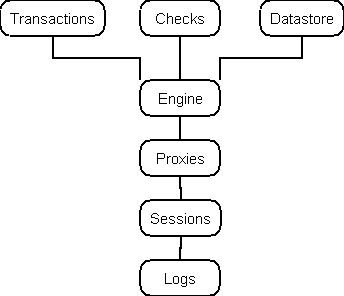
\includegraphics[scale=0.45]{arch.png}

\section{Adding to checks}
\index{Checks!Adding to existing}
Many checks rely on simple text configuration files that can be easily edited to 
increase coverage.

For instance, the bad\_directory check searches all of the seen directories for accessible
subdirectories that are generally undesirable such as 'backup' or 'IISAdmin'.
If you want to add a directory to the bad\_directory check, all you have to do
is edit modules/bad\_directory.cfg and add the directory you want the tool to search for.
\lstinputlisting[style=config]{../modules/bad_directories.cfg}

The config file format is quite simple but flexible. 
\footnote{ProxMon uses http://www.red-dove.com/python\_config.html by Vinay Sajip}
If you want a simple string, just type it with no quotes.  Single or double
quotes will generally ensure proper escaping.  Anything after a \# is a comment.

A more complicated example is the bad\_files check.  This check is run in online mode 
and checks all detected directories for common problem files such as test scripts, 
configuration files that might contain sensitive information or known vulnerable scripts.
\lstinputlisting[style=config]{../modules/bad_files.cfg}

Another useful feature of ProxMon is that it can tell you what frameworks are in 
use.  For instance, the version of PHP\footnote{http://www.php.net} or 
YUI\footnote{http://developer.yahoo.com/yui}.  These tests require a little more
sophistication when specifying strings.  This module allows the use of regular
expressions so you can be fairly accurate.  
\lstinputlisting[style=config]{../modules/id_framework_passive.cfg}

\section{Writing checks}
\index{Checks!Writing}
You can add your own checks to allow ProxMon to understand a custom application, or 
make it aware of a security issue you are particularly concerned about. If your 
application always enforces a certain page flow, ProxMon could have a custom check 
that verifies this flow is consistent. It could also attempt to perform actions 
without sending the correct cookies or modify request values illegally. This can make 
ProxMon a valuable part of your regression testing process.  

All you need to do to have ProxMon incorporate your check is to place the
new check in the modules subdirectory and ProxMon will automatically detect it if 
it's a subclass of pmcheck.

\subsection{Passive checks}
\index{Checks!Passive}
Here's a module that does nothing.
\lstinputlisting[style=code]{../modules/nop.py}

The first line references the file that contains the class definitions for the
check classes.  The check class is the base class and it is used for most passive
checks.  The netcheck class is used for active checks, anything that will make 
outbound network connections should subclass from this.  The last basic check 
type is the postruncheck, which is only run at the end of a session and is used
by the cookie\_summary check and query\_summary checks.

The above check doesn't do anything because it doesn't implement any functions
that are automatically run during or after transaction processing.

Most checks are based on the check class and, as mentioned above, run when the 
full transaction has finished processing and all data is available.  To run like 
this, just declare a function called run()
\lstinputlisting[style=code]{../modules/secure_cookies_sent_clear.py}

Here the module is checking pmd (which is the ProxMon Datastore).  This is
updated constantly with information on values seen in the various transactions.

The SetCookieSecureValues dictionary is keyed by value.  To find out if any
value is also seen clear, all you have to do is loop through the keys in
the dictionary and compare against those in pmd's ClearValues dictionary.

Knowing that isn't enough to get output though.  A call to the check class's
add\_single() method is needed for the application to report on the issue.

Other methods are available.  For instance, the req\_hl\_parse method is
called anytime there's a request header line available to process.
\lstinputlisting[style=code]{../modules/http_auth.py}

Since all this check is concerned with is the request headers, there's no need
to implement a run() function.  The simple presence of an Authorization header
is information enough.

\subsection{Check methods}
The following is in the same order as the methods would be called during
normal transaction processing.
\subsubsection{Called from transaction.parserequest}
\begin{mindesc}
\item[rl\_parse()] Parses the first line of the request\\
This contains the method ('GET', 'HEAD', ...), the requested URL 
('http://www.isecpartners.com:80/index.html') and the HTTP version ('HTTP/1.0')
\item[req\_hl\_parse()] Called for each header line\\
This is passed the whole header line ('Host: www.isecpartners.com$\backslash$r$\backslash$n')
\item[req\_body\_parse()] Called to parse the full body\\
This is generally the POST or PUT contents
\end{mindesc}
\subsubsection{Called from transaction.parseresponse}
\begin{mindesc}
\item[sl\_parse()] Parses the first line of the response. (The status line)\\
('200 OK HTTP/1.0')
\item[resp\_hl\_parse()] Called for each header line\\
Similar to the request Headers
\item[resp\_body\_parse()] Called on the uncompressed response body.\\
The code in transaction.py will handle gzip and both varieties of deflate.
\end{mindesc}
\subsubsection{Called from proxmon.scan or proxmon.tail}
\begin{mindesc}
\item[run()] The full transaction has been handled and the transaction 
dictionary is fully populated.  All values will have been added to the datastore.
\end{mindesc}

\subsection{Active checks}
\index{Checks!Active}
Checks that do more than just parse the stored transactions are also quite easy
to write.  These checks allow you to actively test for classes of vulnerabilities
that can't be detected by parsing log files alone.

The urltesting module has a number of convenient functions available
that will connect out to target hosts and check for or retrieve files.  This
module is based on curl \footnote{http://curl.haxx.se/} and pyCurl
\footnote{http://pycurl.sourceforge.net/}.

If your network check uses the functions in urltesting and you are on a network that 
requires the use of a proxy (other than WebScarab), it will automatically use the
proxy specified in the http\_proxy and https\_proxy environment variables
or you can override these via the -p command line parameter.  It will also get 
access to the appropriate cookies, which are constantly written out as
proxmon.cj in Mozilla cookies.txt format.

The expiry on cookies stored to the proxmon.cj file are incorrect.  In order
to ensure the availability of ephemeral cookies or ones with a very short
lifetime, the expiry is changed to 1 year after the current time.

\lstinputlisting[style=code]{../modules/dir_listing.py}

This module waits until transaction processing is complete and then iterates
through any unseen transactions.  First, it expands the path to include any
implied directories (eg /foo/bar/baz/ implies /, /foo, /foo/bar/).  Then
it searches through any that it hasn't seen already and sees if they contain
strings that imply that the directory contents are viewable.

Important to note is the difference between t['server'] and t['host'].
'server' contains the hostname and port (such as isecpartners.com:80), whereas 
host just includes the name or IP of the server (simply isecpartners.com).  You 
generally want to be careful when writing checks to reference
the former instead of the latter.  Different systems are often running on 
different ports or under different server names.  Distinguishing by 'host'
alone isn't always sufficient.

\subsection{Transaction properties}
Given a normal request for http://www.isecpartners.com:80/index.html?a=1\&b=2 the values
the transaction dictionary would have are given in ().  The following is in the order the
properties are added.
\subsubsection{Assigned by the proxy module}
\begin{mindesc}
\item[id] The transaction identifier (1)
\end{mindesc}
\subsubsection{Assigned in transaction.py by parsereqline()}
\begin{mindesc}
%\item[request] The full request as one string (GET http://www.isec ...)
%\item[response] The full response as one string (200 OK HTTP/1.1\\r\\nHost: www ...)
\item[method] The HTTP method used in the request ('GET')
\item[url] The full URL ('http://www.isecpartners.com:80/index.html?a=1\&b=2') 
\item[version] The HTTP Version ('HTTP/1.0') 
\item[proto] Either http or https ('http')
\item[hostname] Just the host portion of the URL ('www.isecpartners.com')
\item[domain] The last 2 or 3 portions of the hostname ('isecpartners.com')
\item[qsf] The full query string ('a=1\&b=2')
\item[qs] A list with the portions of the QS ('[\{'name': 'a', 'value': '1'\} ... ]')
\item[path] Server side directory ('/')
\item[port] Port the server is listening on ('80') 
\item[server] The combined hostname and port ('www.isecpartners.com:80')
\end{mindesc}
\subsubsection{Assigned in transaction.py by parserequest()}
\begin{mindesc}
\item[sentcookies] A list of cookies sent by the client
\item[host] The Host: header value
\end{mindesc}
\subsubsection{Assigned in transaction.py by parserequest()}
\begin{mindesc}
\item[setcookies] A list of cookies set by the server, complete with flags
\item[respcontenttype] The value of the Content-Type header
\item[respcontentlength] The value of the Content-Length header
\item[location] The value of the Location header
\end{mindesc}


\section{Datastore}
Currently the datastore is focused on tracking values that are seen in cookies, 
on the query string or are sent as post parameters.  These are all set by the 
transaction module.

Each of these values has the associated transaction details (described above) 
available under the 'httpparams' key.

\subsection{Lists}
\begin{mindesc}
\item[Transactions] All processed transactions
\item[SetCookies] All cookies seen in SetCookie headers
\item[SentCookies] All cookies seen in Cookie headers\
\item[QueryStrings] All values passed on the query string
\item[PostParams] All values sent via POST
\end{mindesc}

\subsection{Dictionaries (keyed by value)}
\begin{mindesc}
\item[SetCookieValues] All Set-Cookies
\item[SetCookieSSLValues] Set-Cookies sent over SSL
\item[SetCookieSecureValues] Set-Cookies with the Secure flag\
\item[SentCookieValues] All values sent in Cookie headers from the client
\item[AllCookieValues] All of the cookies
\item[QueryStringValues] All values sent via the query string
\item[QuerySPostParamValues] All values submitted in POSTs
\item[ClearValues] All values sent cleartext
\item[SecureValues] All values sent over SSL
\item[AllValues] Everything
\end{mindesc}

\section{Supporting Other Proxies}
Adding support for other proxies is fairly straight forward.  The full interface is
documented in the appendicies, but partially repeated here so that readers can get
an idea of the process.
\subsection{Methods}
New proxy modules must support the following methods:
\begin{mindesc}
\item[sessions(where)] Gets a list of available sessions, this is populated via the session\_info() function
\item[session\_info(where, name)] Returns a dict including the session id, whether the session is still active, a list of domains seen in the session, a list of transactions (only required to contain the request and status lines) and dates.
\item[get(session, tinfo)] Returns the specified transaction from the selected session\\
get() and get\_next only have to be able to pass the request and response bodies as strings 
to the engine in order to take advantage of the appropriate processing code in transaction.py.
\item[get\_next(session)] Returns the next unseen transaction
\end{mindesc}

\subsection{Variables}
New proxy modules must also define the following variables:
\begin{mindesc}
\item[proxy\_name] The string that will be displayed by the engine
\end{mindesc}

\pagebreak
\appendix
\include{latex/pmcheck-module}
\include{latex/pmdata-module}
\include{latex/urltesting-module}
\include{latex/transaction-module}
\include{latex/pmproxy-module}

\printindex
\end{document}
